% U-Net
% Made with Xematics. Positions are in px (1 px = 0.75 pt), as in the SVG export.
\documentclass[tikz, border=4pt]{standalone}
\definecolor{xm1}{HTML}{FFFFFF}
\definecolor{xm2}{HTML}{6B7280}
\definecolor{xm3}{HTML}{D4E8F5}
\definecolor{xm4}{HTML}{0072B2}
\definecolor{xm5}{HTML}{F1F2F4}
\definecolor{xm6}{HTML}{4B5563}
\definecolor{xm7}{HTML}{DFE3E8}
\definecolor{xm8}{HTML}{FBE8C4}
\definecolor{xm9}{HTML}{B97800}
\definecolor{xm10}{HTML}{AEB3B9}
\definecolor{xm11}{HTML}{2F7FB5}
\definecolor{xm12}{HTML}{1F2937}
\begin{document}
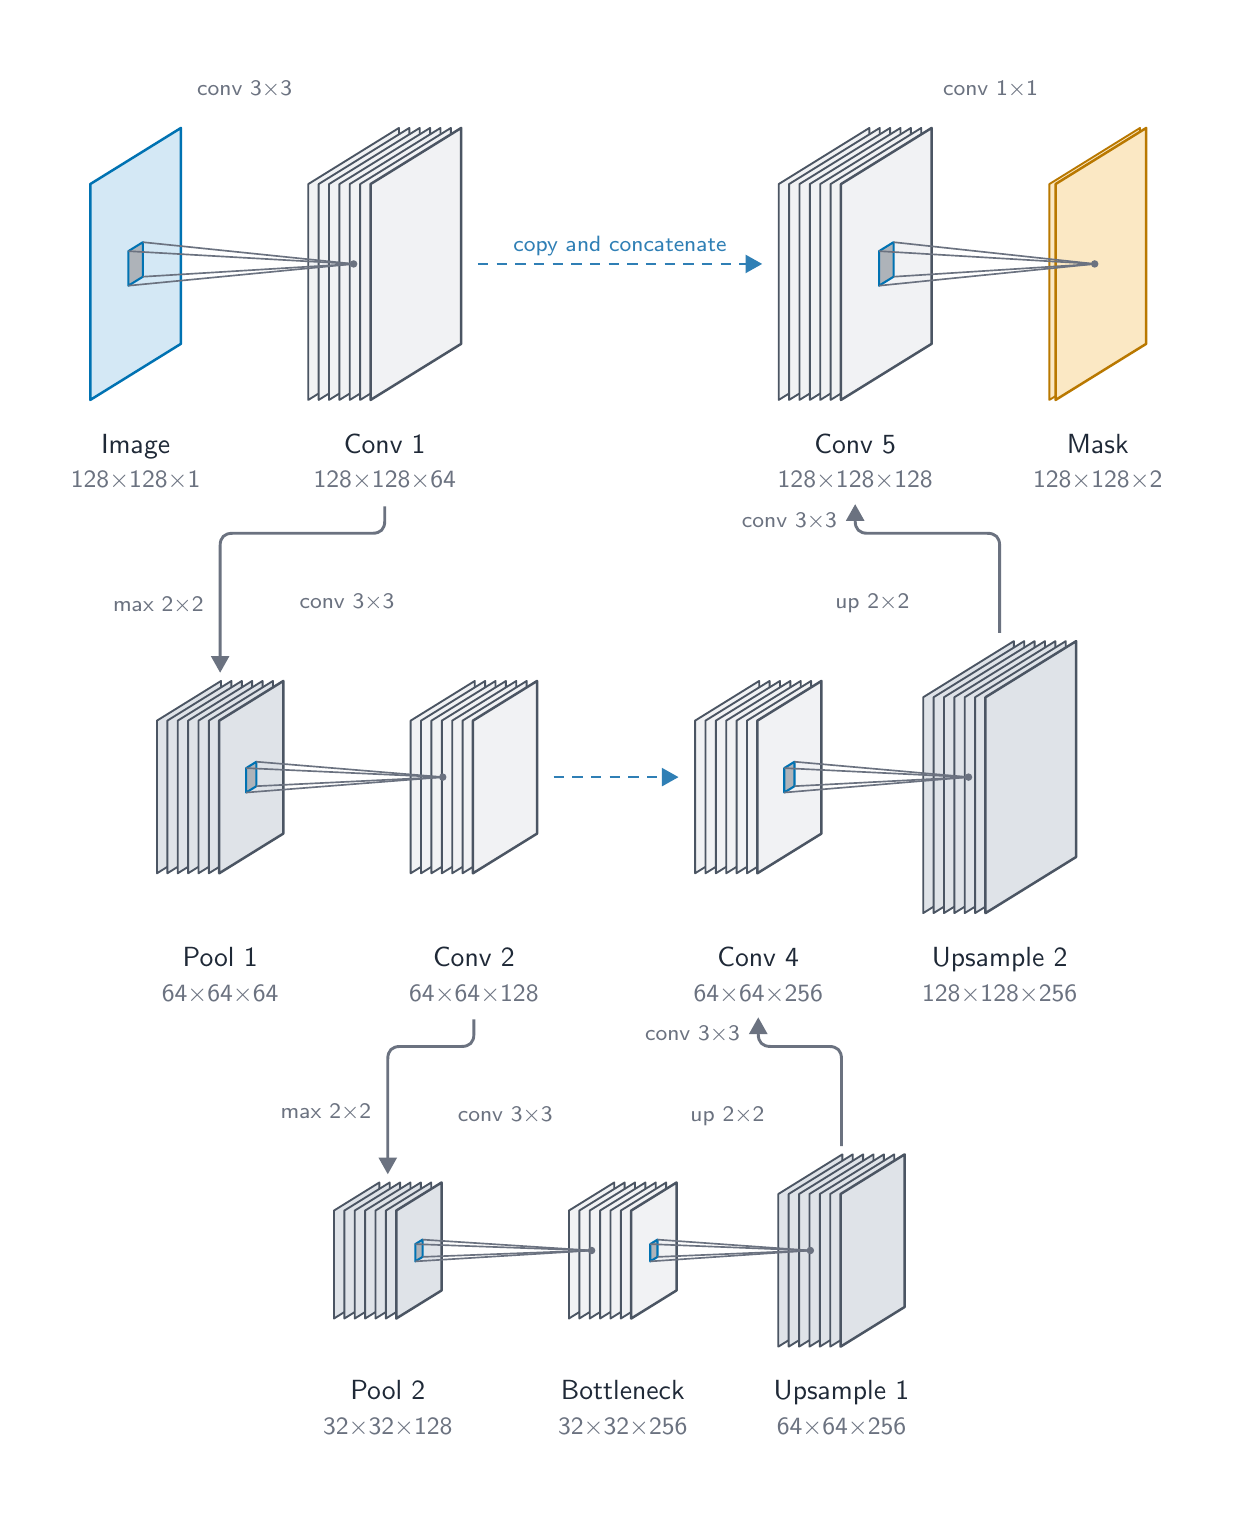
\begin{tikzpicture}[x=0.75pt, y=-0.75pt]
  \tikzset{
    xm elbow/.style={fill=none, draw=xm2, line width=1.05pt, line join=round},
    xm arrow head/.style={fill=xm2},
    xm map input/.style={fill=xm3, draw=xm4, line width=0.9pt, line join=round},
    xm map hidden back/.style={fill=xm5, draw=xm6, line width=0.68pt, line join=round},
    xm map hidden/.style={fill=xm5, draw=xm6, line width=0.9pt, line join=round},
    xm map pool back/.style={fill=xm7, draw=xm6, line width=0.68pt, line join=round},
    xm map pool/.style={fill=xm7, draw=xm6, line width=0.9pt, line join=round},
    xm map output back/.style={fill=xm8, draw=xm9, line width=0.68pt, line join=round},
    xm map output/.style={fill=xm8, draw=xm9, line width=0.9pt, line join=round},
    xm window/.style={fill=xm10, draw=xm4, line width=0.75pt, line join=round},
    xm ray/.style={draw=xm2, line width=0.6pt},
    xm ray end/.style={fill=xm2},
    xm bridge/.style={fill=none, draw=xm11, line width=0.98pt, dash pattern=on 3.75pt off 3pt, line join=round},
    xm bridge head/.style={fill=xm11},
    xm bridge xm11/.style={text=xm11, inner sep=0, font=\sffamily\fontsize{8.25}{9.9}\selectfont},
    xm name xm12/.style={text=xm12, inner sep=0, font=\sffamily\fontsize{9.75}{11.7}\selectfont},
    xm size xm2/.style={text=xm2, inner sep=0, font=\sffamily\fontsize{9}{10.8}\selectfont},
    xm op xm2/.style={text=xm2, inner sep=0, font=\sffamily\fontsize{8.25}{9.9}\selectfont},
  }
  \fill[xm1] (0,0) rectangle (568.81,702.73);
  % Connections 1
  \draw[xm elbow] (172.04,230.6) -- (172.04,237.6) .. controls (172.04,241.6) and (170.04,243.6) .. (166.04,243.6) -- (98.73,243.6) .. controls (94.73,243.6) and (92.73,245.6) .. (92.73,249.6) -- (92.73,303.75);
  \fill[xm arrow head] (92.73,310.75) -- (88.23,302.75) -- (97.23,302.75) -- cycle;
  % Connections 3
  \draw[xm elbow] (214.98,477.85) -- (214.98,484.85) .. controls (214.98,488.85) and (212.98,490.85) .. (208.98,490.85) -- (179.5,490.85) .. controls (175.5,490.85) and (173.5,492.85) .. (173.5,496.85) -- (173.5,545.39);
  \fill[xm arrow head] (173.5,552.39) -- (169,544.39) -- (178,544.39) -- cycle;
  % Connections 6
  \draw[xm elbow] (392.09,538.82) -- (392.09,496.85) .. controls (392.09,492.85) and (390.09,490.85) .. (386.09,490.85) -- (357.99,490.85) .. controls (353.99,490.85) and (351.99,488.85) .. (351.99,484.85) -- (351.99,483.85);
  \fill[xm arrow head] (351.99,476.85) -- (356.49,484.85) -- (347.49,484.85) -- cycle;
  % Connections 8
  \draw[xm elbow] (468.3,291.56) -- (468.3,249.6) .. controls (468.3,245.6) and (466.3,243.6) .. (462.3,243.6) -- (404.69,243.6) .. controls (400.69,243.6) and (398.69,241.6) .. (398.69,237.6) -- (398.69,236.6);
  \fill[xm arrow head] (398.69,229.6) -- (403.19,237.6) -- (394.19,237.6) -- cycle;
  % Layers
  \draw[xm map input] (30.16,75.35) -- (73.84,48.31) -- (73.84,152.31) -- (30.16,179.35) -- cycle;
  \draw[xm map hidden back] (135.2,75.35) -- (178.88,48.31) -- (178.88,152.31) -- (135.2,179.35) -- cycle;
  \draw[xm map hidden back] (140.2,75.35) -- (183.88,48.31) -- (183.88,152.31) -- (140.2,179.35) -- cycle;
  \draw[xm map hidden back] (145.2,75.35) -- (188.88,48.31) -- (188.88,152.31) -- (145.2,179.35) -- cycle;
  \draw[xm map hidden back] (150.2,75.35) -- (193.88,48.31) -- (193.88,152.31) -- (150.2,179.35) -- cycle;
  \draw[xm map hidden back] (155.2,75.35) -- (198.88,48.31) -- (198.88,152.31) -- (155.2,179.35) -- cycle;
  \draw[xm map hidden back] (160.2,75.35) -- (203.88,48.31) -- (203.88,152.31) -- (160.2,179.35) -- cycle;
  \draw[xm map hidden] (165.2,75.35) -- (208.88,48.31) -- (208.88,152.31) -- (165.2,179.35) -- cycle;
  \draw[xm map pool back] (62.29,333.87) -- (93.17,314.75) -- (93.17,388.29) -- (62.29,407.41) -- cycle;
  \draw[xm map pool back] (67.29,333.87) -- (98.17,314.75) -- (98.17,388.29) -- (67.29,407.41) -- cycle;
  \draw[xm map pool back] (72.29,333.87) -- (103.17,314.75) -- (103.17,388.29) -- (72.29,407.41) -- cycle;
  \draw[xm map pool back] (77.29,333.87) -- (108.17,314.75) -- (108.17,388.29) -- (77.29,407.41) -- cycle;
  \draw[xm map pool back] (82.29,333.87) -- (113.17,314.75) -- (113.17,388.29) -- (82.29,407.41) -- cycle;
  \draw[xm map pool back] (87.29,333.87) -- (118.17,314.75) -- (118.17,388.29) -- (87.29,407.41) -- cycle;
  \draw[xm map pool] (92.29,333.87) -- (123.17,314.75) -- (123.17,388.29) -- (92.29,407.41) -- cycle;
  \draw[xm map hidden back] (184.53,333.87) -- (215.42,314.75) -- (215.42,388.29) -- (184.53,407.41) -- cycle;
  \draw[xm map hidden back] (189.53,333.87) -- (220.42,314.75) -- (220.42,388.29) -- (189.53,407.41) -- cycle;
  \draw[xm map hidden back] (194.53,333.87) -- (225.42,314.75) -- (225.42,388.29) -- (194.53,407.41) -- cycle;
  \draw[xm map hidden back] (199.53,333.87) -- (230.42,314.75) -- (230.42,388.29) -- (199.53,407.41) -- cycle;
  \draw[xm map hidden back] (204.53,333.87) -- (235.42,314.75) -- (235.42,388.29) -- (204.53,407.41) -- cycle;
  \draw[xm map hidden back] (209.53,333.87) -- (240.42,314.75) -- (240.42,388.29) -- (209.53,407.41) -- cycle;
  \draw[xm map hidden] (214.53,333.87) -- (245.42,314.75) -- (245.42,388.29) -- (214.53,407.41) -- cycle;
  \draw[xm map pool back] (147.58,569.91) -- (169.42,556.39) -- (169.42,608.39) -- (147.58,621.91) -- cycle;
  \draw[xm map pool back] (152.58,569.91) -- (174.42,556.39) -- (174.42,608.39) -- (152.58,621.91) -- cycle;
  \draw[xm map pool back] (157.58,569.91) -- (179.42,556.39) -- (179.42,608.39) -- (157.58,621.91) -- cycle;
  \draw[xm map pool back] (162.58,569.91) -- (184.42,556.39) -- (184.42,608.39) -- (162.58,621.91) -- cycle;
  \draw[xm map pool back] (167.58,569.91) -- (189.42,556.39) -- (189.42,608.39) -- (167.58,621.91) -- cycle;
  \draw[xm map pool back] (172.58,569.91) -- (194.42,556.39) -- (194.42,608.39) -- (172.58,621.91) -- cycle;
  \draw[xm map pool] (177.58,569.91) -- (199.42,556.39) -- (199.42,608.39) -- (177.58,621.91) -- cycle;
  \draw[xm map hidden back] (260.78,569.91) -- (282.62,556.39) -- (282.62,608.39) -- (260.78,621.91) -- cycle;
  \draw[xm map hidden back] (265.78,569.91) -- (287.62,556.39) -- (287.62,608.39) -- (265.78,621.91) -- cycle;
  \draw[xm map hidden back] (270.78,569.91) -- (292.62,556.39) -- (292.62,608.39) -- (270.78,621.91) -- cycle;
  \draw[xm map hidden back] (275.78,569.91) -- (297.62,556.39) -- (297.62,608.39) -- (275.78,621.91) -- cycle;
  \draw[xm map hidden back] (280.78,569.91) -- (302.62,556.39) -- (302.62,608.39) -- (280.78,621.91) -- cycle;
  \draw[xm map hidden back] (285.78,569.91) -- (307.62,556.39) -- (307.62,608.39) -- (285.78,621.91) -- cycle;
  \draw[xm map hidden] (290.78,569.91) -- (312.62,556.39) -- (312.62,608.39) -- (290.78,621.91) -- cycle;
  \draw[xm map pool back] (361.65,561.94) -- (392.53,542.82) -- (392.53,616.36) -- (361.65,635.48) -- cycle;
  \draw[xm map pool back] (366.65,561.94) -- (397.53,542.82) -- (397.53,616.36) -- (366.65,635.48) -- cycle;
  \draw[xm map pool back] (371.65,561.94) -- (402.53,542.82) -- (402.53,616.36) -- (371.65,635.48) -- cycle;
  \draw[xm map pool back] (376.65,561.94) -- (407.53,542.82) -- (407.53,616.36) -- (376.65,635.48) -- cycle;
  \draw[xm map pool back] (381.65,561.94) -- (412.53,542.82) -- (412.53,616.36) -- (381.65,635.48) -- cycle;
  \draw[xm map pool back] (386.65,561.94) -- (417.53,542.82) -- (417.53,616.36) -- (386.65,635.48) -- cycle;
  \draw[xm map pool] (391.65,561.94) -- (422.53,542.82) -- (422.53,616.36) -- (391.65,635.48) -- cycle;
  \draw[xm map hidden back] (321.55,333.87) -- (352.44,314.75) -- (352.44,388.29) -- (321.55,407.41) -- cycle;
  \draw[xm map hidden back] (326.55,333.87) -- (357.44,314.75) -- (357.44,388.29) -- (326.55,407.41) -- cycle;
  \draw[xm map hidden back] (331.55,333.87) -- (362.44,314.75) -- (362.44,388.29) -- (331.55,407.41) -- cycle;
  \draw[xm map hidden back] (336.55,333.87) -- (367.44,314.75) -- (367.44,388.29) -- (336.55,407.41) -- cycle;
  \draw[xm map hidden back] (341.55,333.87) -- (372.44,314.75) -- (372.44,388.29) -- (341.55,407.41) -- cycle;
  \draw[xm map hidden back] (346.55,333.87) -- (377.44,314.75) -- (377.44,388.29) -- (346.55,407.41) -- cycle;
  \draw[xm map hidden] (351.55,333.87) -- (382.44,314.75) -- (382.44,388.29) -- (351.55,407.41) -- cycle;
  \draw[xm map pool back] (431.46,322.6) -- (475.14,295.56) -- (475.14,399.56) -- (431.46,426.6) -- cycle;
  \draw[xm map pool back] (436.46,322.6) -- (480.14,295.56) -- (480.14,399.56) -- (436.46,426.6) -- cycle;
  \draw[xm map pool back] (441.46,322.6) -- (485.14,295.56) -- (485.14,399.56) -- (441.46,426.6) -- cycle;
  \draw[xm map pool back] (446.46,322.6) -- (490.14,295.56) -- (490.14,399.56) -- (446.46,426.6) -- cycle;
  \draw[xm map pool back] (451.46,322.6) -- (495.14,295.56) -- (495.14,399.56) -- (451.46,426.6) -- cycle;
  \draw[xm map pool back] (456.46,322.6) -- (500.14,295.56) -- (500.14,399.56) -- (456.46,426.6) -- cycle;
  \draw[xm map pool] (461.46,322.6) -- (505.14,295.56) -- (505.14,399.56) -- (461.46,426.6) -- cycle;
  \draw[xm map hidden back] (361.85,75.35) -- (405.53,48.31) -- (405.53,152.31) -- (361.85,179.35) -- cycle;
  \draw[xm map hidden back] (366.85,75.35) -- (410.53,48.31) -- (410.53,152.31) -- (366.85,179.35) -- cycle;
  \draw[xm map hidden back] (371.85,75.35) -- (415.53,48.31) -- (415.53,152.31) -- (371.85,179.35) -- cycle;
  \draw[xm map hidden back] (376.85,75.35) -- (420.53,48.31) -- (420.53,152.31) -- (376.85,179.35) -- cycle;
  \draw[xm map hidden back] (381.85,75.35) -- (425.53,48.31) -- (425.53,152.31) -- (381.85,179.35) -- cycle;
  \draw[xm map hidden back] (386.85,75.35) -- (430.53,48.31) -- (430.53,152.31) -- (386.85,179.35) -- cycle;
  \draw[xm map hidden] (391.85,75.35) -- (435.53,48.31) -- (435.53,152.31) -- (391.85,179.35) -- cycle;
  \draw[xm map output back] (492.25,75.35) -- (535.93,48.31) -- (535.93,152.31) -- (492.25,179.35) -- cycle;
  \draw[xm map output] (495.24,75.35) -- (538.92,48.31) -- (538.92,152.31) -- (495.24,179.35) -- cycle;
  \draw[xm window] (48.51,107.67) -- (55.5,103.35) -- (55.5,119.99) -- (48.51,124.31) -- cycle;
  \draw[xm ray] (48.51,107.67) -- (157.04,113.83);
  \draw[xm ray] (55.5,103.35) -- (157.04,113.83);
  \draw[xm ray] (55.5,119.99) -- (157.04,113.83);
  \draw[xm ray] (48.51,124.31) -- (157.04,113.83);
  \fill[xm ray end] (157.04,113.83) circle[radius=1.8];
  \draw[xm window] (105.26,356.73) -- (110.2,353.67) -- (110.2,365.44) -- (105.26,368.5) -- cycle;
  \draw[xm ray] (105.26,356.73) -- (199.98,361.08);
  \draw[xm ray] (110.2,353.67) -- (199.98,361.08);
  \draw[xm ray] (110.2,365.44) -- (199.98,361.08);
  \draw[xm ray] (105.26,368.5) -- (199.98,361.08);
  \fill[xm ray end] (199.98,361.08) circle[radius=1.8];
  \draw[xm window] (186.75,586.07) -- (190.25,583.91) -- (190.25,592.23) -- (186.75,594.39) -- cycle;
  \draw[xm ray] (186.75,586.07) -- (271.7,589.15);
  \draw[xm ray] (190.25,583.91) -- (271.7,589.15);
  \draw[xm ray] (190.25,592.23) -- (271.7,589.15);
  \draw[xm ray] (186.75,594.39) -- (271.7,589.15);
  \fill[xm ray end] (271.7,589.15) circle[radius=1.8];
  \draw[xm window] (299.95,586.07) -- (303.45,583.91) -- (303.45,592.23) -- (299.95,594.39) -- cycle;
  \draw[xm ray] (299.95,586.07) -- (377.09,589.15);
  \draw[xm ray] (303.45,583.91) -- (377.09,589.15);
  \draw[xm ray] (303.45,592.23) -- (377.09,589.15);
  \draw[xm ray] (299.95,594.39) -- (377.09,589.15);
  \fill[xm ray end] (377.09,589.15) circle[radius=1.8];
  \draw[xm window] (364.52,356.73) -- (369.46,353.67) -- (369.46,365.44) -- (364.52,368.5) -- cycle;
  \draw[xm ray] (364.52,356.73) -- (453.3,361.08);
  \draw[xm ray] (369.46,353.67) -- (453.3,361.08);
  \draw[xm ray] (369.46,365.44) -- (453.3,361.08);
  \draw[xm ray] (364.52,368.5) -- (453.3,361.08);
  \fill[xm ray end] (453.3,361.08) circle[radius=1.8];
  \draw[xm window] (410.19,107.67) -- (417.18,103.35) -- (417.18,119.99) -- (410.19,124.31) -- cycle;
  \draw[xm ray] (410.19,107.67) -- (514.09,113.83);
  \draw[xm ray] (417.18,103.35) -- (514.09,113.83);
  \draw[xm ray] (417.18,119.99) -- (514.09,113.83);
  \draw[xm ray] (410.19,124.31) -- (514.09,113.83);
  \fill[xm ray end] (514.09,113.83) circle[radius=1.8];
  % Skip connections
  \draw[xm bridge] (216.88,113.83) -- (346.85,113.83);
  \fill[xm bridge head] (353.85,113.83) -- (345.85,118.33) -- (345.85,109.33) -- cycle;
  \draw[xm bridge] (253.42,361.08) -- (306.55,361.08);
  \fill[xm bridge head] (313.55,361.08) -- (305.55,365.58) -- (305.55,356.58) -- cycle;
  % Labels
  \node[xm bridge xm11, anchor=base] at (285.37,107.83) {copy and concatenate};
  \node[xm name xm12, anchor=base] at (52,204.94) {Image};
  \node[xm size xm2, anchor=base] at (52,221.7) {128\ensuremath{\times}128\ensuremath{\times}1};
  \node[xm op xm2, anchor=base] at (104.52,32.66) {conv 3\ensuremath{\times}3};
  \node[xm name xm12, anchor=base] at (172.04,204.94) {Conv 1};
  \node[xm size xm2, anchor=base] at (172.04,221.7) {128\ensuremath{\times}128\ensuremath{\times}64};
  \node[xm op xm2, anchor=base] at (62.93,281.18) {max 2\ensuremath{\times}2};
  \node[xm name xm12, anchor=base] at (92.73,452.2) {Pool 1};
  \node[xm size xm2, anchor=base] at (92.73,468.96) {64\ensuremath{\times}64\ensuremath{\times}64};
  \node[xm op xm2, anchor=base] at (153.85,279.91) {conv 3\ensuremath{\times}3};
  \node[xm name xm12, anchor=base] at (214.98,452.2) {Conv 2};
  \node[xm size xm2, anchor=base] at (214.98,468.96) {64\ensuremath{\times}64\ensuremath{\times}128};
  \node[xm op xm2, anchor=base] at (143.7,525.62) {max 2\ensuremath{\times}2};
  \node[xm name xm12, anchor=base] at (173.5,661.07) {Pool 2};
  \node[xm size xm2, anchor=base] at (173.5,677.83) {32\ensuremath{\times}32\ensuremath{\times}128};
  \node[xm op xm2, anchor=base] at (230.1,527.17) {conv 3\ensuremath{\times}3};
  \node[xm name xm12, anchor=base] at (286.7,661.07) {Bottleneck};
  \node[xm size xm2, anchor=base] at (286.7,677.83) {32\ensuremath{\times}32\ensuremath{\times}256};
  \node[xm op xm2, anchor=base] at (337.13,527.17) {up 2\ensuremath{\times}2};
  \node[xm name xm12, anchor=base] at (392.09,661.07) {Upsample 1};
  \node[xm size xm2, anchor=base] at (392.09,677.83) {64\ensuremath{\times}64\ensuremath{\times}256};
  \node[xm op xm2, anchor=base] at (320.31,487.85) {conv 3\ensuremath{\times}3};
  \node[xm name xm12, anchor=base] at (351.99,452.2) {Conv 4};
  \node[xm size xm2, anchor=base] at (351.99,468.96) {64\ensuremath{\times}64\ensuremath{\times}256};
  \node[xm op xm2, anchor=base] at (406.95,279.91) {up 2\ensuremath{\times}2};
  \node[xm name xm12, anchor=base] at (468.3,452.2) {Upsample 2};
  \node[xm size xm2, anchor=base] at (468.3,468.96) {128\ensuremath{\times}128\ensuremath{\times}256};
  \node[xm op xm2, anchor=base] at (367.01,240.6) {conv 3\ensuremath{\times}3};
  \node[xm name xm12, anchor=base] at (398.69,204.94) {Conv 5};
  \node[xm size xm2, anchor=base] at (398.69,221.7) {128\ensuremath{\times}128\ensuremath{\times}128};
  \node[xm op xm2, anchor=base] at (463.89,32.66) {conv 1\ensuremath{\times}1};
  \node[xm name xm12, anchor=base] at (515.58,204.94) {Mask};
  \node[xm size xm2, anchor=base] at (515.58,221.7) {128\ensuremath{\times}128\ensuremath{\times}2};
\end{tikzpicture}
\end{document}
